\section{Results}
\label{sec:results}
\textbf{Exploration.} Annual DF ranged from 2{,}759 (2017) to 34{,}959 (2020) cases, with large
epidemics in 2013--2014, 2019--2020 and 2022 (Fig.~\ref{fig:cases}). The three surge
definitions pick different weeks: at $h=1$ the Jaccard overlap is 0.31 (A vs S), 0.11 (A vs G)
and 0.05 (S vs G). In the development period (target weeks 2016--2021, 312 weeks) the
prevalence is 13.8\% (A), 14.1\% (S) and 11.5\% (G), but only 7 (A-onset) and 5 (S-onset)
weeks are surges that start from below the threshold.

\begin{table}[ht]
\centering\small
\caption{One-week-ahead results. PR-AUC with 95\% block-bootstrap interval; precision (P) and
recall (R) at the pre-specified alarm threshold $P\ge0.20$. ``Best'' = highest development
PR-AUC among non-baseline models; the same model is then scored on 2022. 2022 intervals are
omitted because 52 weeks hold only two 26-week blocks.}
\label{tab:main}
\begin{tabular}{l r c l c c r c c}
\toprule
 & \multicolumn{5}{c}{Development, target weeks 2016--2021} & \multicolumn{3}{c}{Target weeks 2022}\\
\cmidrule(lr){2-6}\cmidrule(lr){7-9}
Target & Pos. & Persist. & Best model: PR-AUC [95\% CI] & P & R & Pos. & Persist. & Best\\
\midrule
A threshold & 43 & 0.93 & Poisson GLM: 0.93 [0.78, 0.98] & 0.62 & 0.93 & 20 & 0.98 & 0.97\\
S seasonal  & 44 & 0.97 & Ridge log-count: 0.98 [0.77, 1.00] & 0.75 & 1.00 & 27 & 0.98 & 0.97\\
G growth    & 36 & 0.17 & Ridge log-count: 0.26 [0.15, 0.40] & 0.22 & 0.53 & 8 & 0.14 & 0.31\\
A-onset     & 7  & 0.30 & Poisson GLM: 0.32 [0.04, 0.80] & 0.17 & 0.57 & 2 & 0.42 & 0.23\\
S-onset     & 5  & 0.26 & Ridge log-count: 0.89 [0.70, 1.00] & 0.33 & 1.00 & 2 & 0.58 & 1.00\\
\bottomrule
\end{tabular}
\end{table}

\textbf{Development comparison} (Table~\ref{tab:main}, Fig.~\ref{fig:prauc}). For the level
targets A and S, the one-variable persistence baseline (current distance to the threshold)
already reaches PR-AUC 0.93--0.97, and no model beats it reliably: the share of bootstrap
draws in which the best model beats persistence is 0.37 (A) and 0.70 (S). These high scores
mostly mean that a week above the threshold is followed by another one. At the 0.20 threshold
the A model raises about 11 alarms a year and catches 93\% of surge weeks. Growth surges are
hard: the best model (PR-AUC 0.26) is better than persistence (0.17) in 98\% of bootstrap
draws, but it needs about 14 alarms a year to catch half of them. Onset is where count
regression helps most: for S-onset, ridge on log counts reaches 0.89 against 0.26 for
persistence, but this rests on 5 positive weeks. For A-onset no model is clearly useful
(interval 0.04--0.80). At $h=2$ and $h=4$ persistence weakens (A: 0.89, 0.77) and the best
models stay close to it (Appendix figures).

\textbf{Negative results.} Weather alone is weak: the weather-only logistic model scores 0.34
(A), 0.16 (S) and 0.13 (G), close to the base rates of 0.14, 0.14 and 0.12. Adding weather to
case history does not improve on cases alone at $h=1$ (A: 0.89 vs 0.92). Trees are not better
than the linear models (CART 0.77 and random forest 0.84 for A). The lasso keeps some lagged
humidity terms, but given the weak humidity cross-check (Section~\ref{sec:data}) we do not
read this as a weather effect. The count models' one-week-ahead error is MAE 33 cases/week
(RMSE 60) for ridge on log counts, against a development mean of 242 cases/week; at $h=4$ the
MAE is 66.

\textbf{Final period, 2022.} 2022 was Singapore's second-largest year in the series, with
32{,}130 cases. The models chosen on development keep their ranking:
persistence and the selected model score 0.97--0.98 for A and S, and the growth model scores
0.31 against 0.14 for persistence (8 positives). The onset results rest on 2 positives each and
cannot separate models.
\textbf{Failure case.} For A-onset, the Poisson model raised alarms at the June--July 2022 peak.
From the origin 2022-07-04 it predicted 1{,}383 cases ($P=0.52$), but cases fell to 918. The
model extrapolated growth into a turning point. It also missed the onset week of
2022-01-17 ($P=0.18$, just below the alarm threshold).

\textbf{Robustness.} With a one-week reporting delay, PR-AUC for A falls from 0.93 to 0.89
(persistence) and from 0.93 to 0.81 (Poisson GLM); S changes little (0.97 to 0.94). On the
brief's 2014--2018 file (test years 2017--2018), A has 7 positives (logistic 0.80 vs
persistence 0.79), growth has 21 (0.29 vs 0.22), and the seasonal targets have \emph{no}
positives. This file alone cannot evaluate a surge warning, which is why it serves as a
cross-check rather than the main analysis.

\begin{figure}[ht]
  \centering
  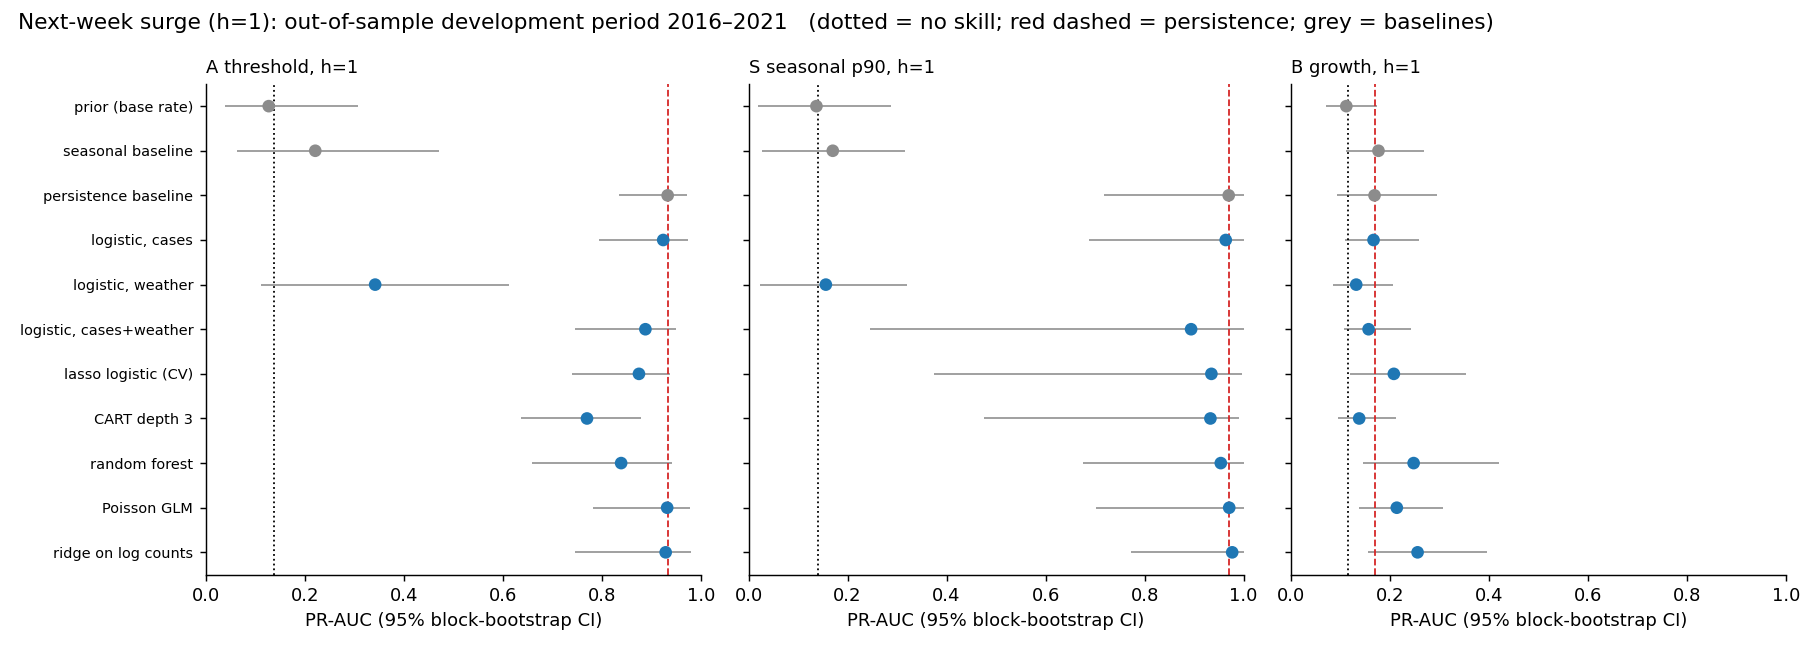
\includegraphics[width=\linewidth]{02_pr_auc_ci_h1.png}
  \caption{Development-period PR-AUC with 95\% block-bootstrap intervals, $h=1$. Dotted line:
  no-skill base rate; red dashed line: persistence baseline.}
  \label{fig:prauc}
\end{figure}
